En este capítulo se presentan los resultados obtenidos al procesar las señales y se realiza un breve análisis. Al registrar sesiones,  se creaba una única sesión y luego se dividía en múltiples partes. Debido a que el posicionamiento del sensor es importante y varía cuando se coloca y se retira,  y a que el estado del cuerpo cambia de un instante al otro, las bioseñales sufren variaciones. Por este motivo, se utilizaban datos de una única sesión tanto como para entrenar como para predecir. De esta manera, se buscaba que la señal sea lo más consistente posible. Para calcular la precisión se utilizó el método de validación cruzada de $k$ iteraciones. Se tomó esta decisión ya que, como se mencionó en la sección \ref{sec:classification}, partir las sesiones en dos partes y utilizar una para entrenamiento y otra para validación no resulta representativo debido a que la elección del lugar en donde se parten los datos puede influir mucho en el resultado. Se utilizaron valores de $k$ iguales a $5$, $10$ y $15$. La elección de estos valores se basó en la cantidad de muestras con la que se contaba. Luego, se promediaban los resultados arrojados por cada valor de $k$ y ese número reflejaba la precisión de la sesión. Tanto en EEG como en EMG se analizaron los siguientes clasificadores: \emph{naive Bayes},  \acrshort{lda}, \gls{svm} y árboles de decisión. En ningún caso se realizó un análisis del por qué algunos clasificadores resultaron mejores que otros ya que no fue el foco de este proyecto.

\section{\acrshort{eeg}} \label{sec:eeg-results}

Como se mencionó en la sección \ref{sec:eeg-signal-processing} del capítulo anterior, primero se comenzó utilizando los valores de potencia \emph{Alfa} que brindaba el sensor ($\alpha_{10 \, Hz}$). Para intentar mejorar la precisión, se decidió realizar una implementación propia ($\alpha_{256 \, Hz}$) y confeccionar el vector de características con cuatro elementos. Para determinar que clasificador utilizar, se utilizaron todos los conjuntos de datos y se promedio la precisión de cada clasificador. En la tabla \ref{tab:eeg-class-result} se pueden observar los resultados de cada clasificador.
 
\begin{table}[H]
\centering
\begin{tabular}{ |c|c|c| } 
 \hline
 Clasificador & Precisión $\alpha_{10 \, Hz}$ &  Precisión $\alpha_{256 \, Hz}$ \\ 
 \hline
 \emph{Naive Bayes} & $0.656$  & $0.615$  \\
 \hline
 \gls{lda}  & $0.667$ & $0.689$ \\
  \hline
  \gls{svm} & $0.627$ & $0.5374$ \\
  \hline
 Árbol de decisión & $0.6723$ & $0.755$ \\
 \hline
\end{tabular}
\caption{Resultados de utilizar distintos clasificadores sobre todas las muestras.}
\label{tab:eeg-class-result}
\end{table}

Se puede observar que los mejores resultados se obtuvieron utilizando un árbol de decisión con un vector de cuatro características obtenido de $256$ muestras. Como en ambos métodos el árbol de decisión fue el que mejores resultados arrojó, se utilizó dicho clasificador.

En la tabla \ref{tab:eeg-results} se pueden observar los resultados de todas las sesiones.

\begin{table}[H]
\centering
\begin{tabular}{ |c|c|c| } 
 \hline
 Sujeto & Precisión $\alpha_{10 \, Hz}$ &  Precisión $\alpha_{256 \, Hz}$ \\ 
 \hline
 1 & $0.565$ & $0.665$ \\
 \hline
 2 & $0.831$ & $0.881$ \\
 \hline
 3 & $0.768$ & $0.881$ \\
 \hline
 4  & $0.727$ & $0.909$ \\
 \hline
  5 & $0.510$ & $0.660$ \\
 \hline
 6 & $0.645$ & $0.655$ \\
 \hline
 7 & $0.656$ & $0.795$ \\
 \hline
 8  & $0.682$ & $0.593$ \\
 \hline

 \hline
\end{tabular}
\caption{Resultados de utilizar distintas formas de calcular potencia de \emph{Alfa} en distintos sujetos utilizando como clasificador un árbol de decisión.}
\label{tab:eeg-results}
\end{table}

La primer observación que se puede realizar es que utilizar $\alpha_{256 \, Hz}$ es más preciso que utilizar $\alpha_{10 \, Hz}$ en la mayoría de los casos. Como se mencionó anteriormente, esto se debe a que en el primer caso se toman $256$ muestras para calcular la potencia de \emph{Alfa} mientras que en el segundo se utilizan únicamente $25$. A su vez, en el primer caso se utilizan los valores obtenidos por cada electrodo por separado mientras que en el segundo caso se promedian y se arma el vector de características con dos valores consecutivos. Utilizar las mediciones de los distintos electrodos en un período de tiempo describe mejor el estado que utilizar valores de dos períodos consecutivos. Se consideró inaceptable que en algunos sujetos la precisión diera muy cercana al azar. Por este motivo y por todo lo mencionado anteriormente, se utilizó el método $\alpha_{256 \, Hz}$.

En las figuras \ref{fig:subject-2-10} y \ref{fig:subject-2-256} se observan gráficos de dispersión utilizando los valores de potencia de \emph{Alfa}. En ambos se observa una clara separación de estados. El estado de ojos cerrados contiene valores mayores que el estado de ojos abiertos. La figura \ref{fig:subject-2-10} cuenta con una cantidad mayor de valores atípicos, particularmente, una cantidad mayor de valores de \emph{Alfa} elevados en el estado de ojos abiertos. A su vez, en la figura \ref{fig:subject-2-256} los valores para ojos abiertos se encuentran mayormente concentrados por debajo de los valores para ojos cerrados. Por estos motivos, la precisión es mayor al utilizar el vector de cuatro dimensiones. Debido a la separación que se observa en los gráficos, fue suficiente utilizar un clasificador simple.

 \begin{figure}[H]
	\centering
    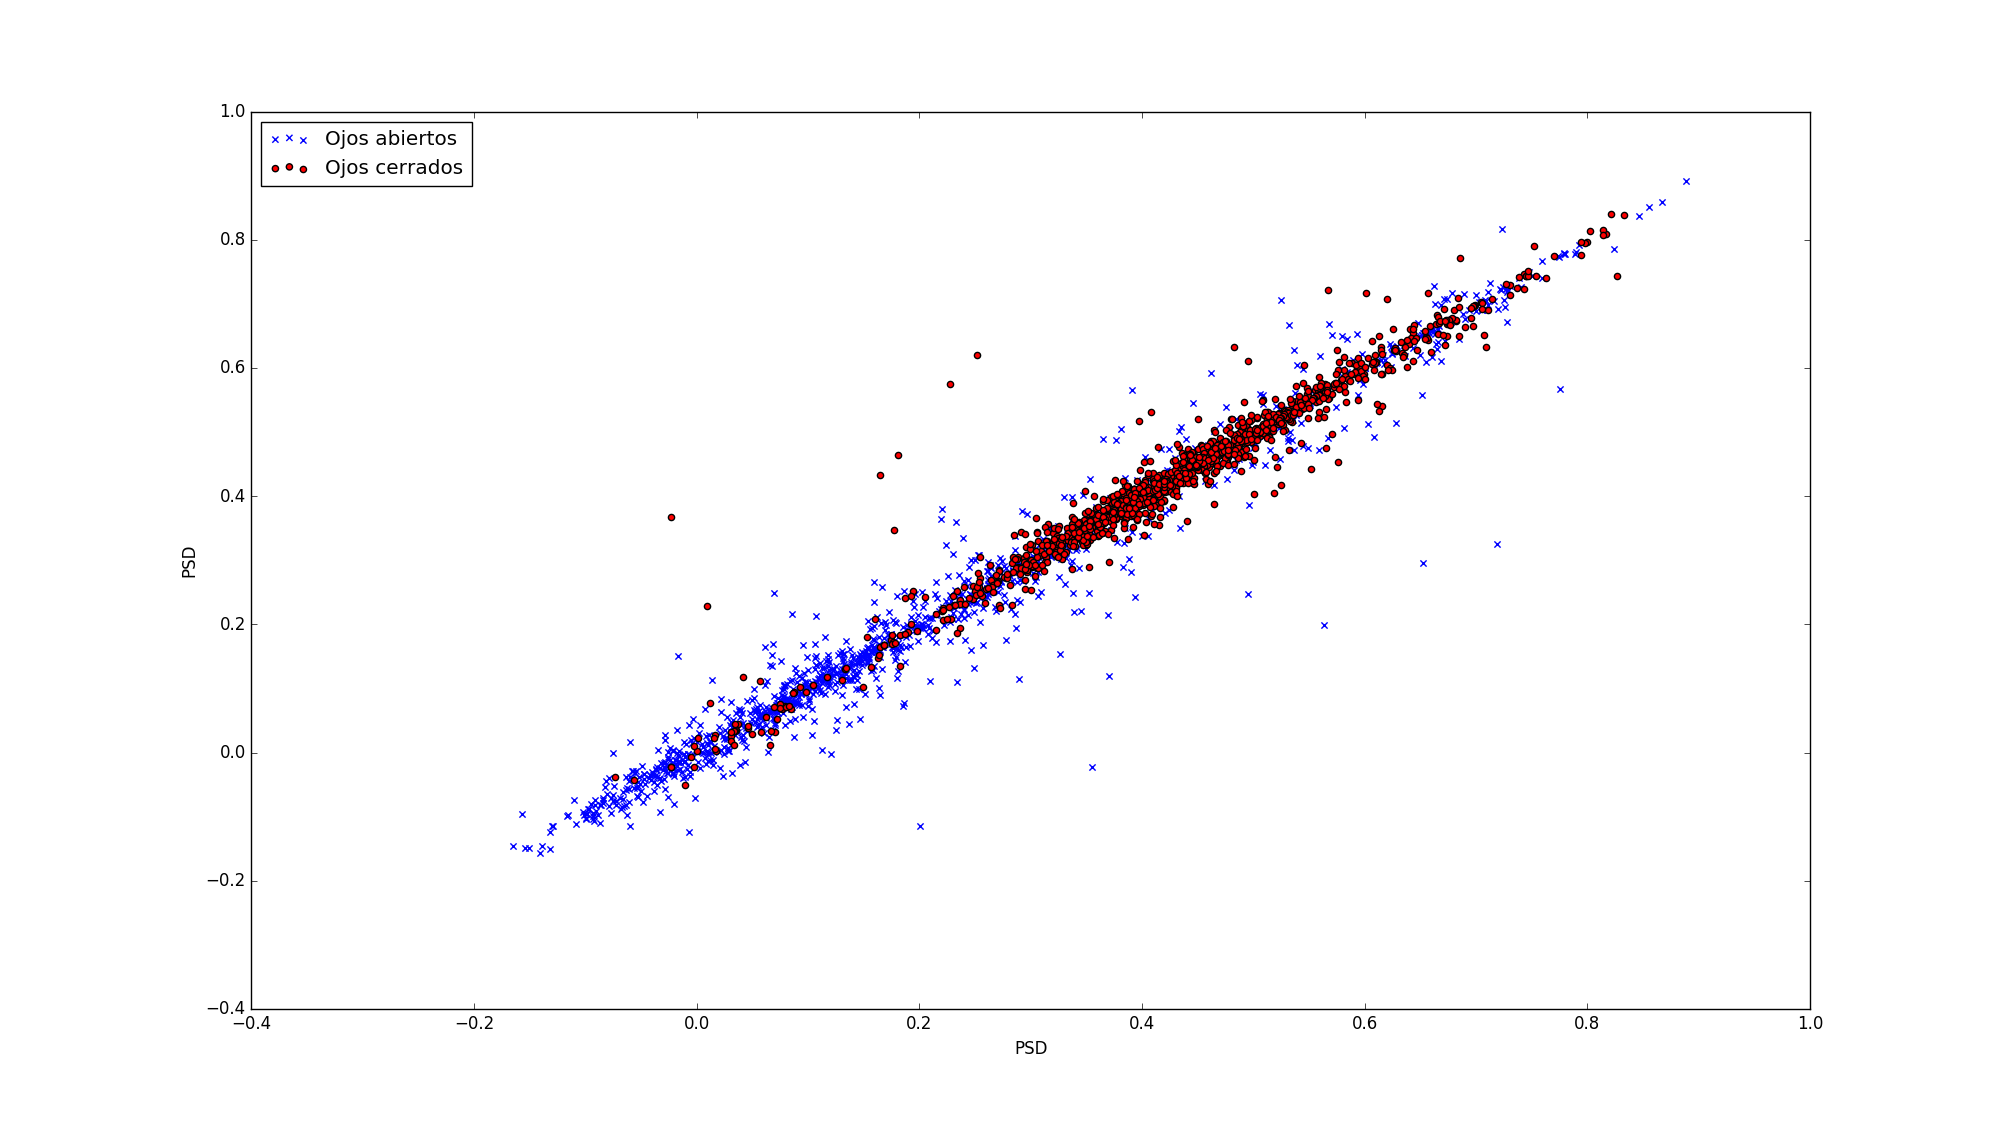
\includegraphics[width=0.8\textwidth]{subject-2-10.png}
    \caption{Gráfico de dispersión del vector de características de dos características del sujeto 2}
	\label{fig:subject-2-10}
\end{figure}

 \begin{figure}[H]
	\centering
    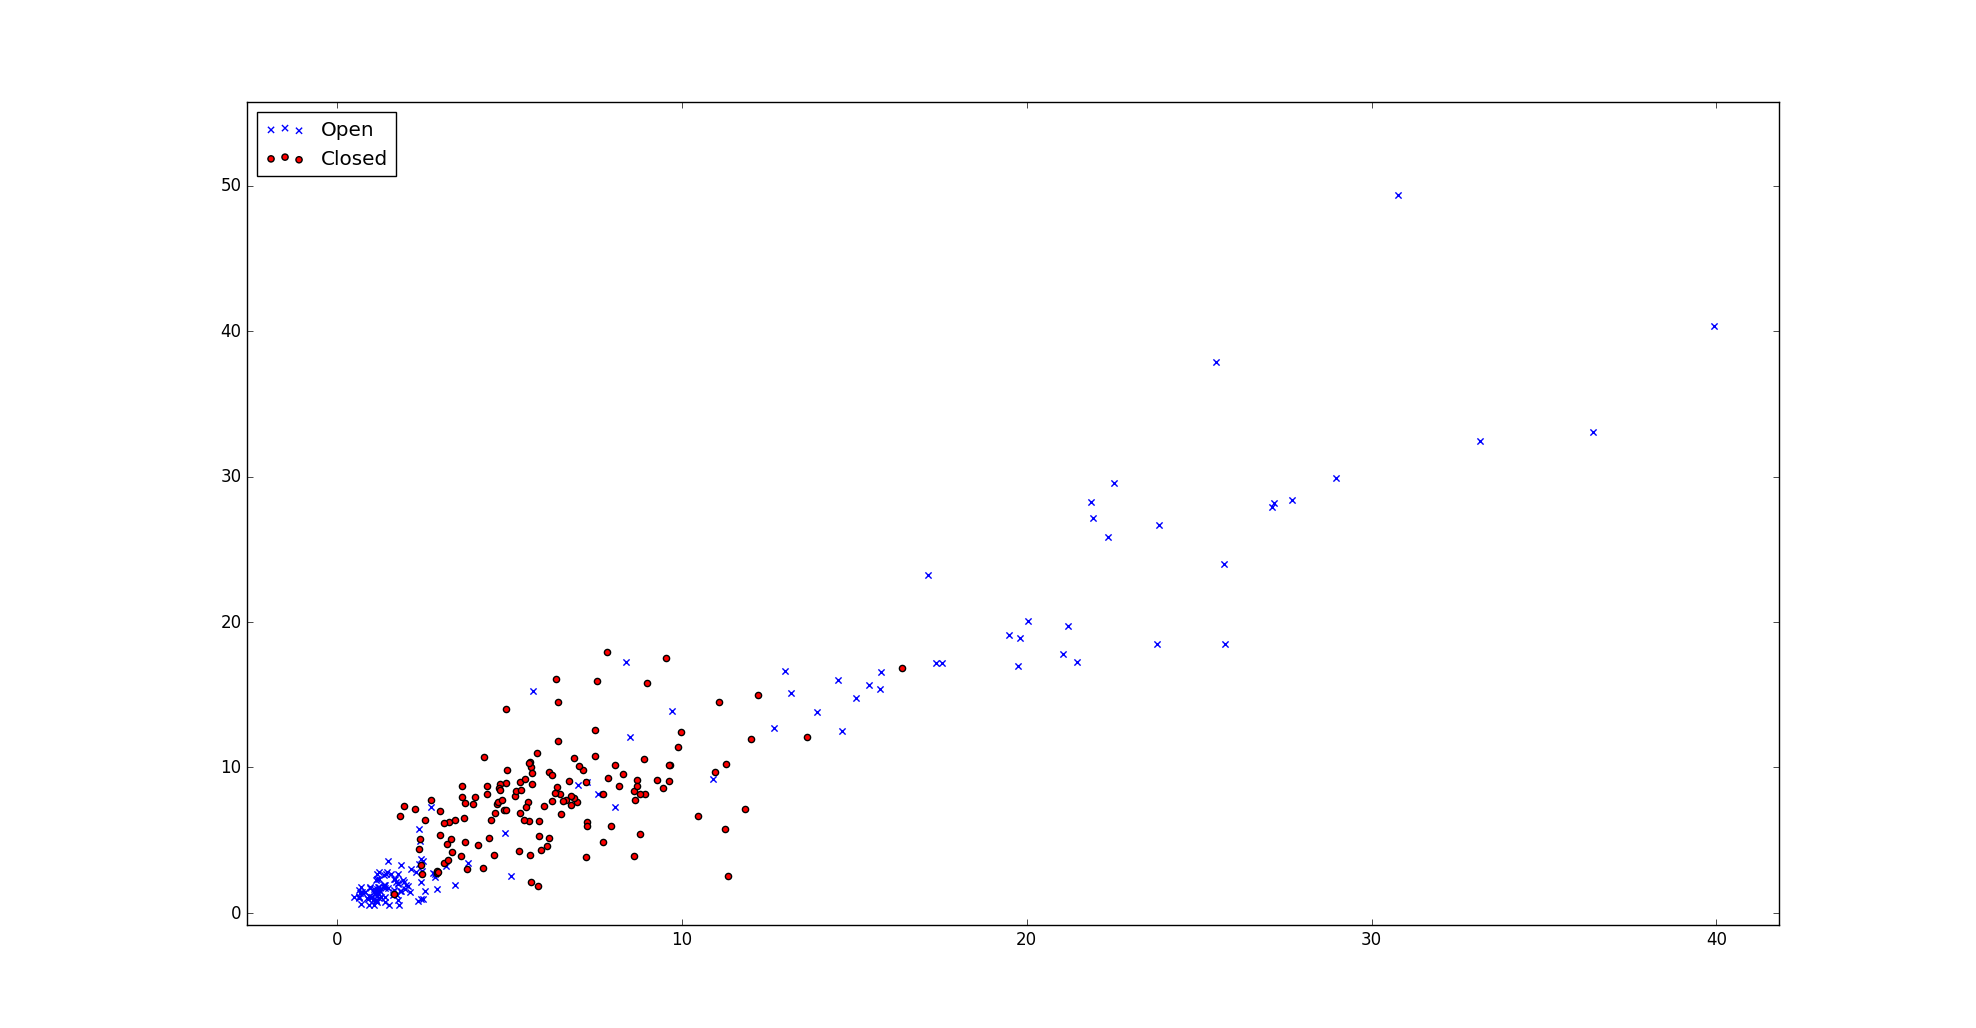
\includegraphics[width=0.8\textwidth]{subject-2-256.png}
    \caption{Gráfico de dispersión del vector de características de cuatro características del sujeto 2. Para transformar de cuatro dimensiones a dos, se promediaron los dos primeros valores y los dos valores finales.}
	\label{fig:subject-2-256}
\end{figure}


Al comparar las figuras \ref{fig:subject-1-256} y \ref{fig:subject-2-256}, se puede observar, que hay una mayor separación entre estados en la figura \ref{fig:subject-2-256}. Por este motivo, la precisión del sujeto $2$ fue un $20\%$ superior.

 \begin{figure}[H]
	\centering
    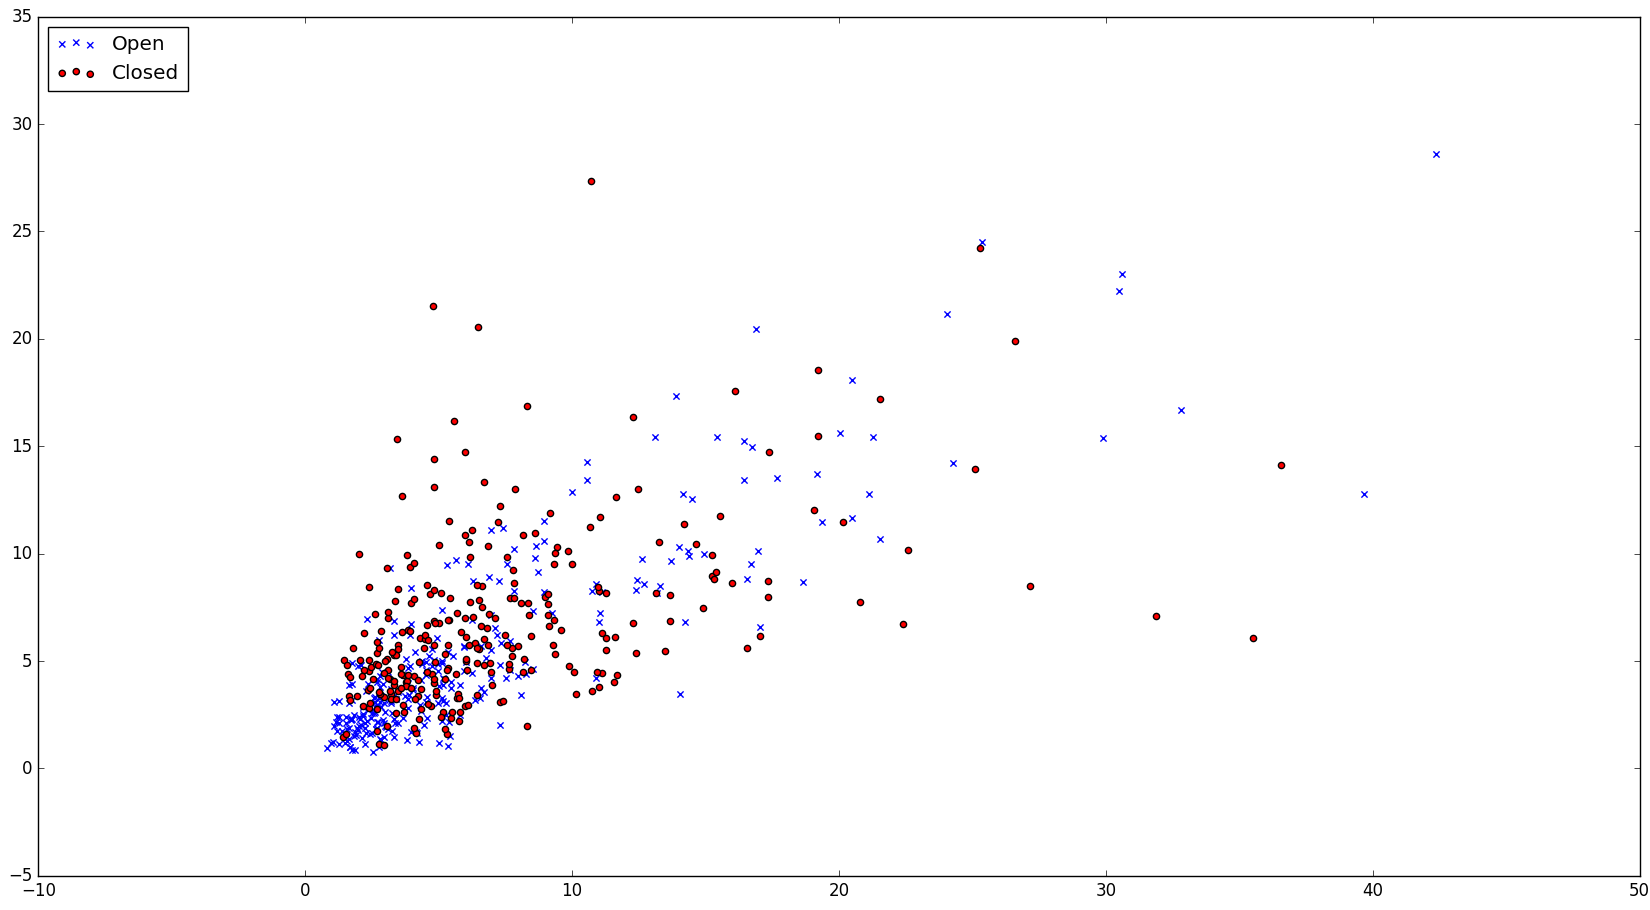
\includegraphics[width=0.8\textwidth]{subject-1-256.png}
    \caption{Gráfico de dispersión del vector de características de cuatro características del sujeto 1.}
	\label{fig:subject-1-256}
\end{figure}

Cabe destacar que al contar con un vector de cuatro características, para graficar se necesitarían cuatro dimensiones. Para abordar este problema se decidió transformar el vector en un vector de dos componentes donde la primer componente es el promedio de los dos primeros valores y la segunda, el promedio de los dos últimos valores.

Otro aspecto a analizar es el hecho de que la precisión varía mucho de sujeto a sujeto, la variación inter-personal intrínseca de cada individuo. Esto puede deberse a diversos motivos, pero generalmente se atribuyen a la variabilidad natural biológica. Muchas bioseñales presentan adicionalmente una variación inter-personal notoria, es decir cambios entre las señales de la misma persona en diferentes momentos.  Además, pueden presentar un fenómeno reflexivo, donde al saber que está siendo analizada cada persona, se encuentra nerviosa, por ejemplo, por lo que puede afectar las ondas cerebrales. A su vez, si la persona se encuentra cansada, por ejemplo, los estímulos al campo visual tienden a ser menores, lo que genera que lo valores de \emph{Alfa} sean mayores. Otro de ellos es que el cerbero de dos personas distintas responde formas diferentes antes los estímulos. Esta gran diferencia puede apreciarse al observar que el Sujeto $1$ obtuvo una precisión mucho menor que el resto de los sujetos.

Si bien las ondas cerebrales varían mucho de persona a persona y de acuerdo al instante del tiempo, se realizó la prueba de utilizar como sesión de entrenamiento una sesión del sujeto 2  y como sesión de predicción una sesión del sujeto 1. Los resultados fueron remarcablemente positivos ya que se obtuvo una precisión de $0.6537$. Este valor no es comparable con los obtenidos anteriormente ya que dichos valores utilizaron validación cruzada y éste simplemente utilizo un conjunto de datos para entrenamiento y otro para validación. De esta forma, se observa que el sistema de clasificación ofrece un aceptable nivel de robustez para esta aplicación.

Utilizar un umbral para determinar si el usuario se encontraba con los ojos cerrados, compensó la falta de precisión del clasificador. Se obtuvieron buenos resultados en el universo interactivo con tan solo $1$ minuto de entrenamiento. Si bien agregó una pequeña latencia, mejoró la robustez del sistema.

\section{\acrshort{emg}} \label{sec:emg-results}

Como se mencionó en la sección \ref{sec:emg-signal-processing}, los valores leídos fueron procesados para obtener un vector de dos características cada $128$ muestras, y luego fueron alimentados a un clasificador. Para la elección de clasificador, se realizaron pruebas sobre cuatro clasificadores distintos. Se tomaron seis sesiones de \acrshort{emg} grabadas, y se aplico la técnica de validación cruzada con $k$ iteraciones ( mencionada en la sección \ref{sec:classification}) por cada clasificador. Los resultados fueron los siguientes:

\begin{table}[H]
\centering
\begin{tabular}{ |c|c| }
 \hline
 Clasificador & Precisión \\ 
 \hline
 \emph{Naive Bayes} & $0.962$ \\
 \hline
 \gls{lda} & $0.951$ \\
 \hline
  \gls{svm} & $0.457$ \\
 \hline
 Árbol de decisión & $0.973$ \\
 
 \hline
\end{tabular}
\caption{Precisiones de distintos clasificadores sobre las sesiones de EMG.}
\label{tab:emg-classifiers}
\end{table}

Como se puede observar en la tabla \ref{tab:emg-classifiers}, los niveles de precisión de todos los clasificadores, excepto el de \acrshort{svm}, fueron muy elevados. Se decidió proceder a utilizar el de Árboles de decisión ya que produjo el resultado más elevado. No se realizaron pruebas adicionales ya que se consideró que el nivel de precisión alcanzado era lo suficientemente alto para fines prácticos de la simulación. Como se observará más adelante, existe una clara separación entre los valores de un estado y el otro por lo que un clasificador simple es más que suficiente. Además, los clasificadores o esquemas más complejos requieren más poder de procesamiento y requieren una gran dedicación de tiempo para determinar los mejores parámetros. Luego de haber elegido el clasificador, se pudo realizar un estudio mas detallado, sesión por sesión. En la siguiente tabla se detalla: el sujeto utilizado, la precision alcanzada luego de entrenar al clasificador, y la duración total en segundos de las muestras tomadas. Para calcular la precisión obtenida en cada sesión, se utilizó nuevamente el método de validación cruzada de $k$ iteraciones.

\begin{table}[H]
\centering
\begin{tabular}{ |c|c|c| } 
 \hline
 Sujeto & Precisión & Duración (Segundos) \\ 
 \hline
 1 & $0.970$ & $603$ \\
  \hline
 2 & $0.955$ & $239$ \\
  \hline
 3 & $0.994$ & $393$ \\

 \hline
\end{tabular}
\caption{Resultados de entrenamientos utilizando lecturas de \acrshort{emg} para distintos sujetos. Frecuencia de muestreo: $256\,Hz$.}
\label{tab:emg-results}
\end{table}

Como muestran los valores de la tabla \ref{tab:emg-results}, los niveles de precisión alcanzados son muy elevados: en las tres sesiones realizadas, se logró un nivel de precisión de $95\%$, o mayor. Es necesario remarcar que al medir señales de \acrshort{emg}, existen varias fuentes de ruido eléctrico, que pueden afectar los valores leídos y por lo tanto perjudicar la precision del entrenador. El efecto neto de éstas fuentes de ruido varía de sesión en sesión, ya que depende de factores como la cantidad de movimiento de los electrodos en relación a la piel, o la presencia de dispositivos que emitan radiación electromagnética\cite{emg-delsys}.

A continuación, se muestran los gráficos de dispersión de las dos sesiones más largas, que permiten visualizar las diferencias entre los vectores de características de ambos estados de tensión de músculo.

 \begin{figure}[H]
	\centering
    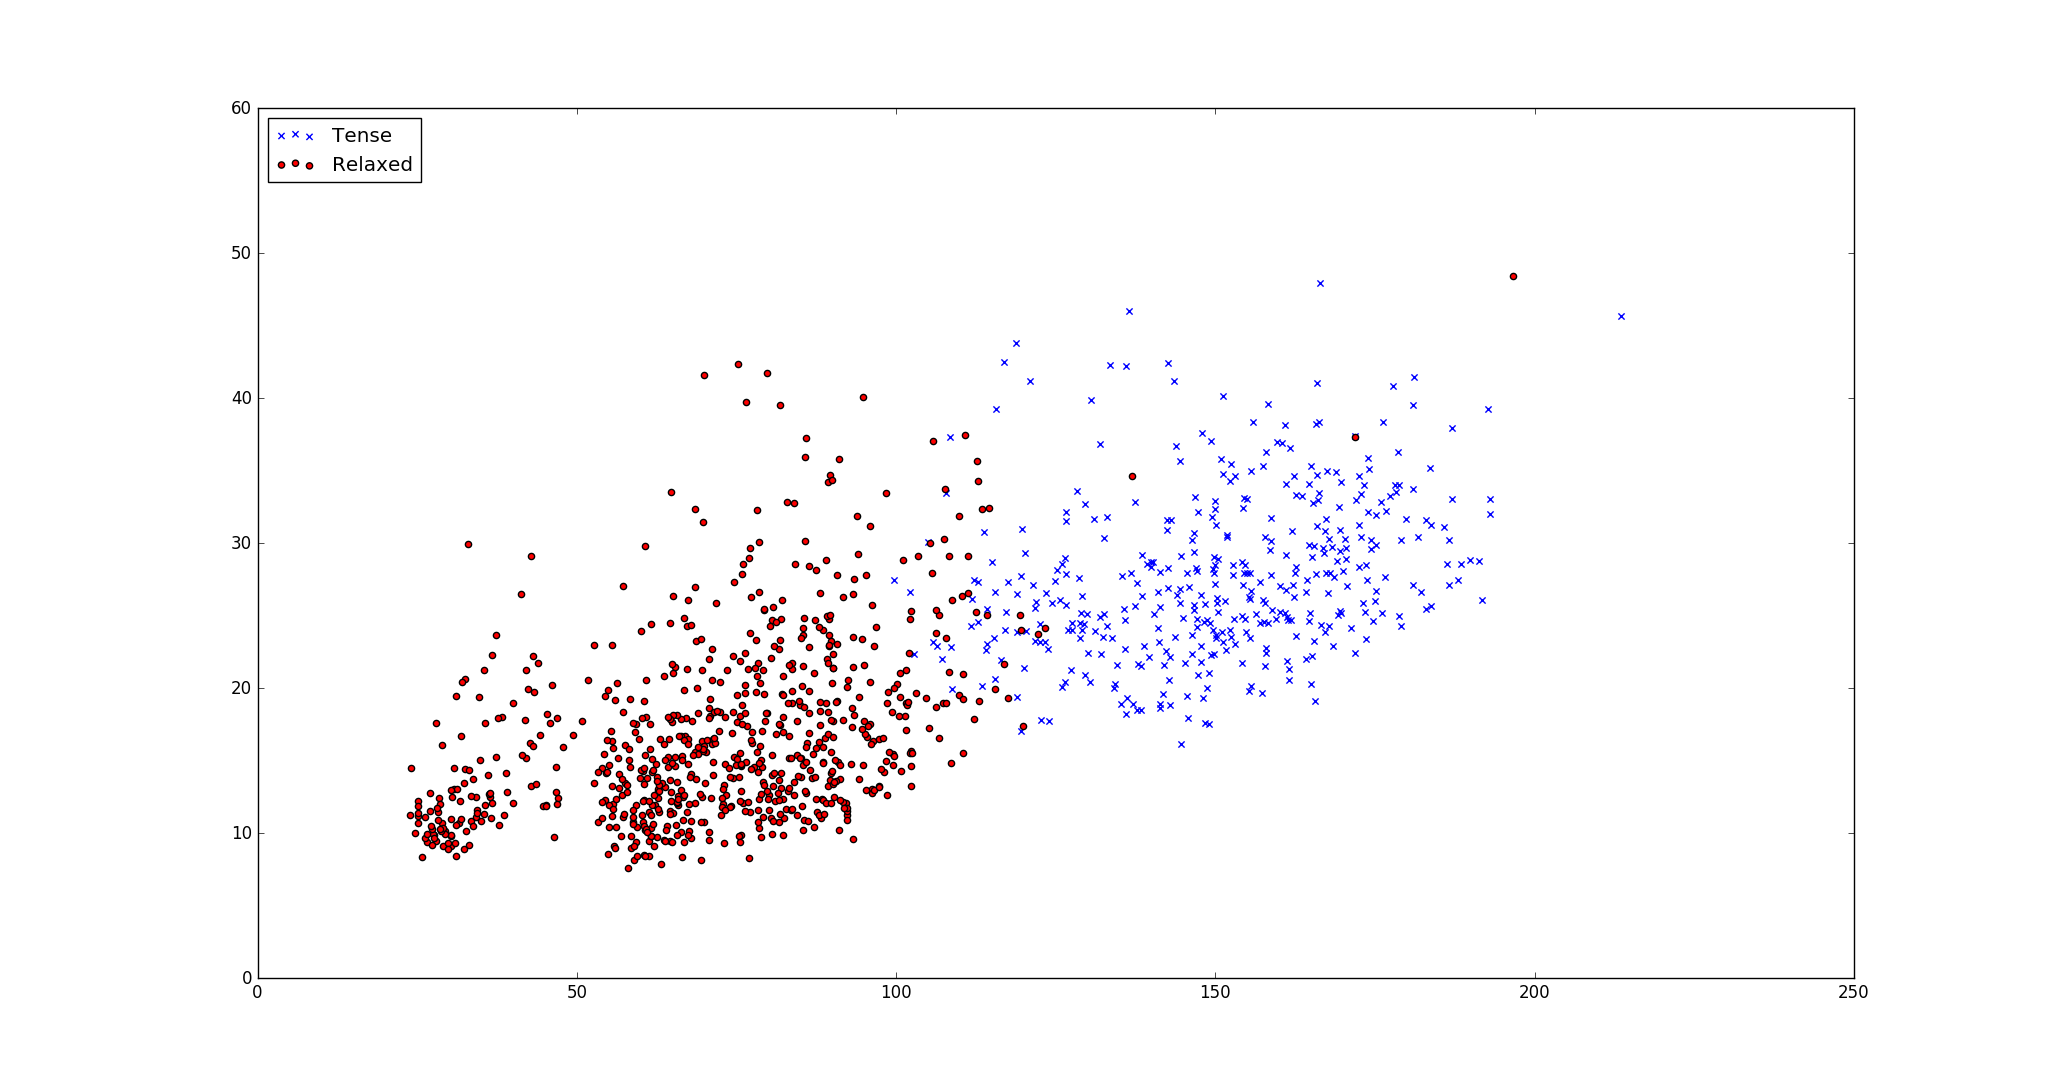
\includegraphics[width=1\textwidth]{fede-1.png}
    \caption{Gráfico de dispersión del vector de características \acrshort{emg} para la sesión del sujeto $1$.}
	\label{fig:emg-graph-s1}
\end{figure}

 \begin{figure}[H]
	\centering
    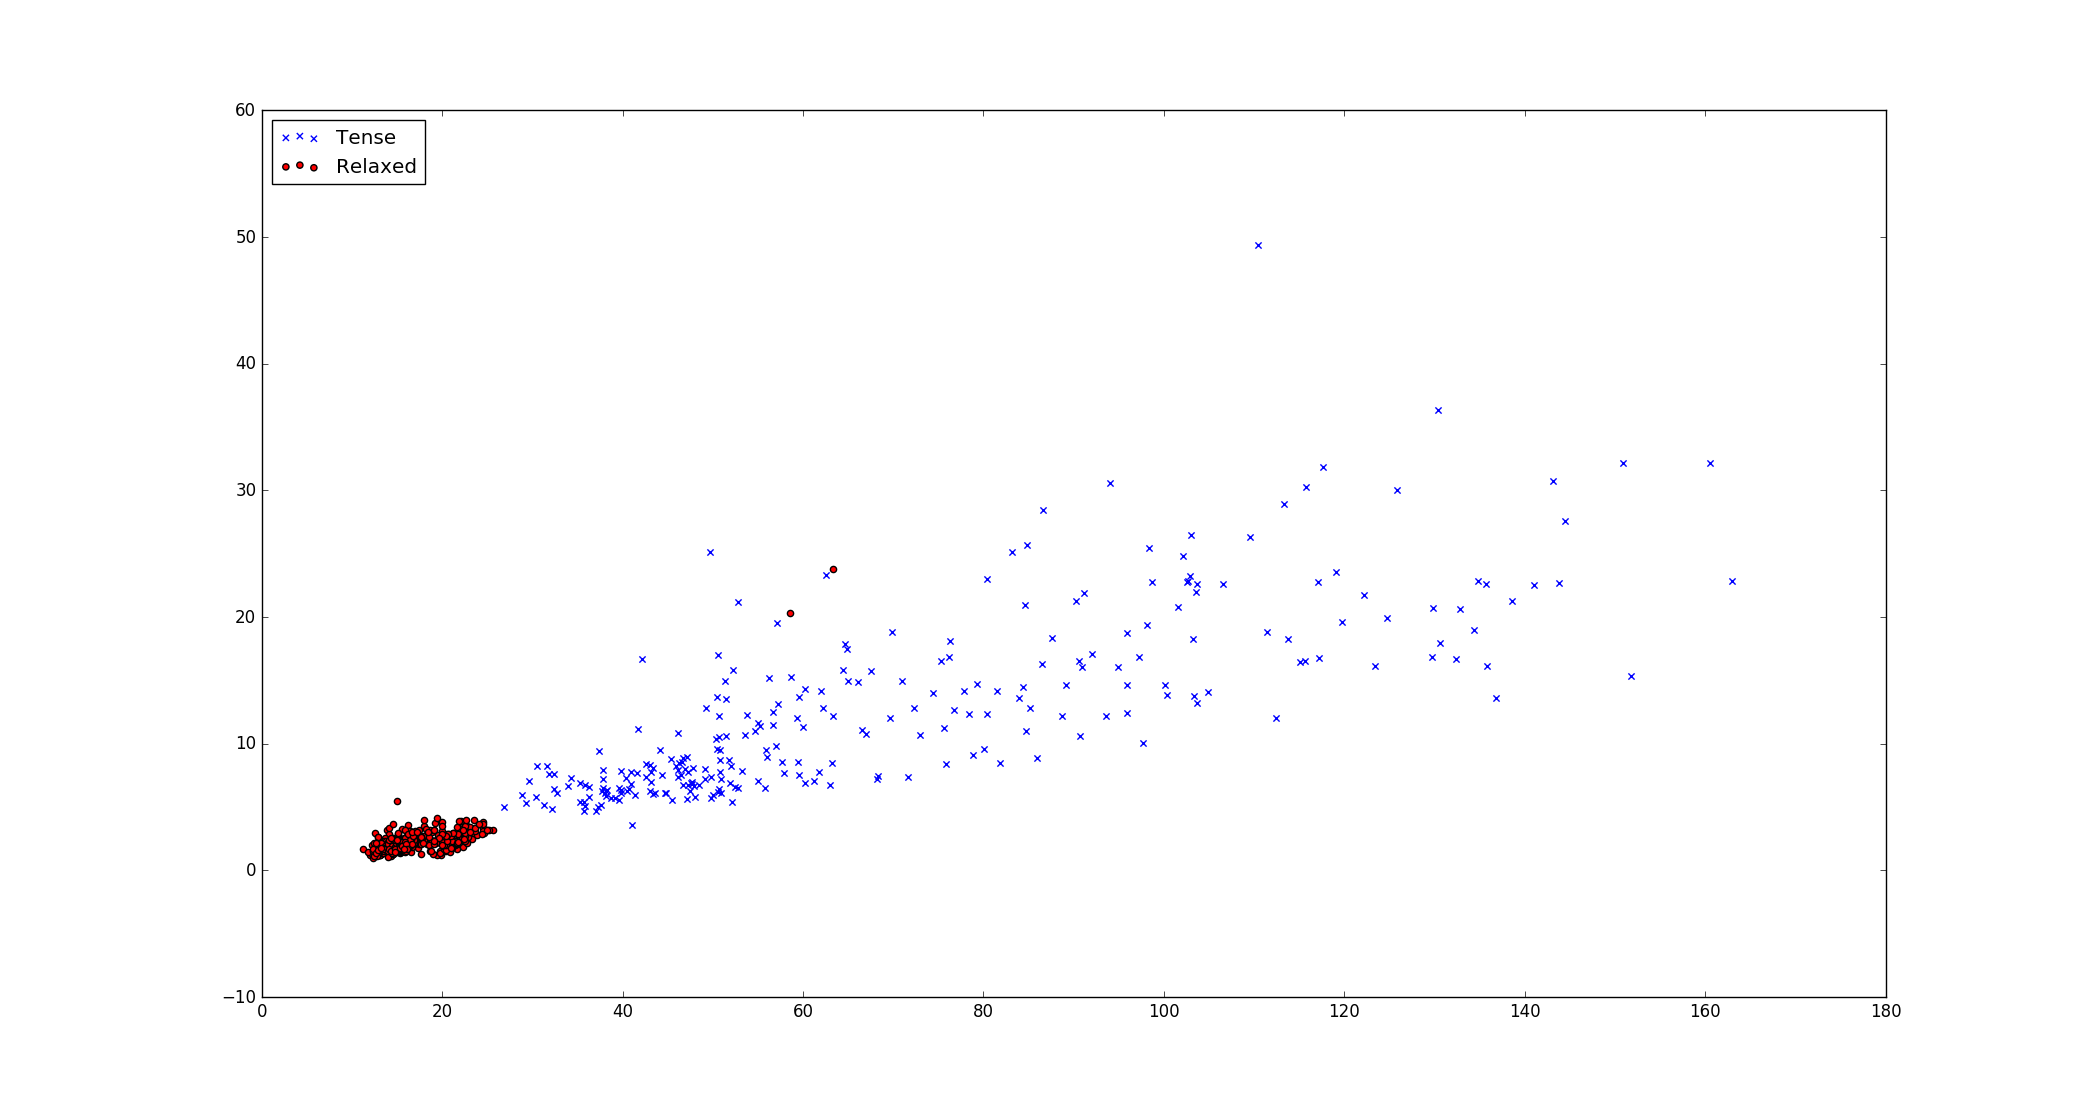
\includegraphics[width=1\textwidth]{javo-1.png}
    \caption{Gráfico de dispersión del vector de características \acrshort{emg} para la sesión del sujeto $3$.}
	\label{fig:emg-graph-s3}
\end{figure}

En la figura \ref{fig:emg-graph-s1}, se puede observar una clara separación entre las muestras tomadas con el musculo relajado, y las muestras tomadas con el musculo tensado. En la figura \ref{fig:emg-graph-s3} se puede observar el mismo efecto, con una separación aun mas marcada. Esta clara separación fue la que permitió utilizar un clasificador simple. También, se puede notar como las muestras tomadas con músculo relajado se encuentran concentradas en un área pequeña, debido a la poca variación de potencial medido de muestra en muestra. Por el otro lado, las muestras tomadas con músculo tensado se encuentran dispersas, ya que al tensar el músculo no siempre es posible mantener el mismo nivel fuerza ejercida.

Como se menciono en la sección \ref{sec:emg-signal-processing}, la frecuencia de muestreo del modulo \acrshort{emg} fue cambiada de $256\,Hz$ a $512\,Hz$. Para comprobar que la precision de predicción se mantuvo luego de este cambio, se grabaron nuevas sesiones.

\begin{table}[H]
\centering
\begin{tabular}{ |c|c|c| } 
 \hline
 Sujeto & Precisión & Duración (Segundos) \\ 
 \hline
 1 & $0.972$ & $284$ \\
 \hline
 2 & $0.991$ & $339$ \\
 \hline
 3 & $0.984$ & $292$ \\
 \hline
 4 & $0.953$ & $130$ \\
 \hline
 5 & $0.969$ & $146$ \\

 \hline
\end{tabular}
\caption{Resultados de entrenamientos utilizando lecturas de \acrshort{emg} para varios sujetos. Frecuencia de muestreo: $512\,Hz$.}
\label{tab:emg-results-512}
\end{table}
	
Como se puede observar en la tabla \ref{tab:emg-results-512}, el nivel de precision se mantuvo elevado, luego de haber realizado el cambio de frecuencia de muestreo. Las dos sesiones mas largas fueron graficadas, nuevamente, para poder observar la relación entre los valores de los vectores de características y el estado del músculo:

\begin{figure}[H]
	\centering
    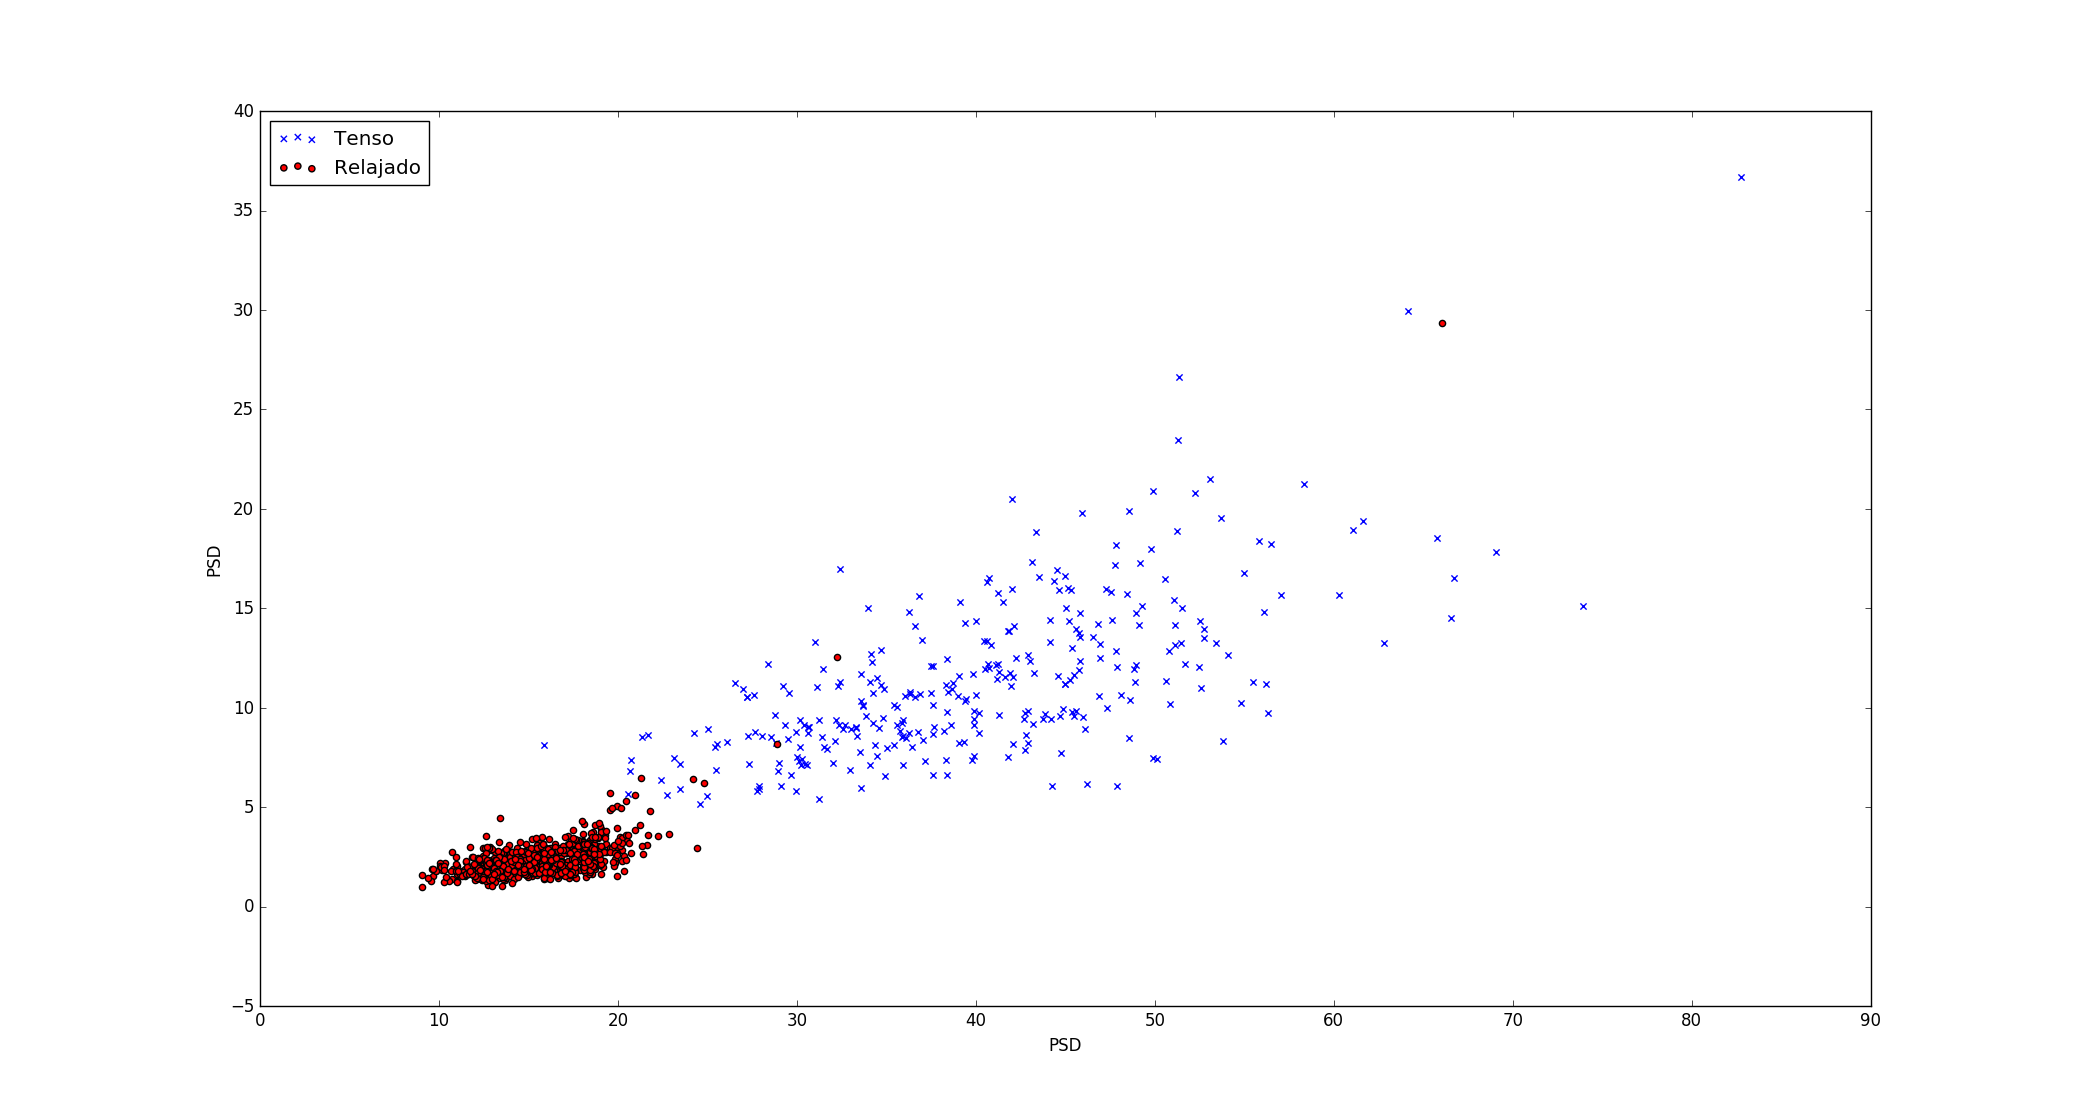
\includegraphics[width=1\textwidth]{fede-512-1.png}
    \caption{Gráfico de dispersión del vector de características EMG para la sesión del sujeto $1$ ($512\,Hz$).}
	\label{fig:emg-graph-s1-512}
\end{figure}

\begin{figure}[H]
	\centering
    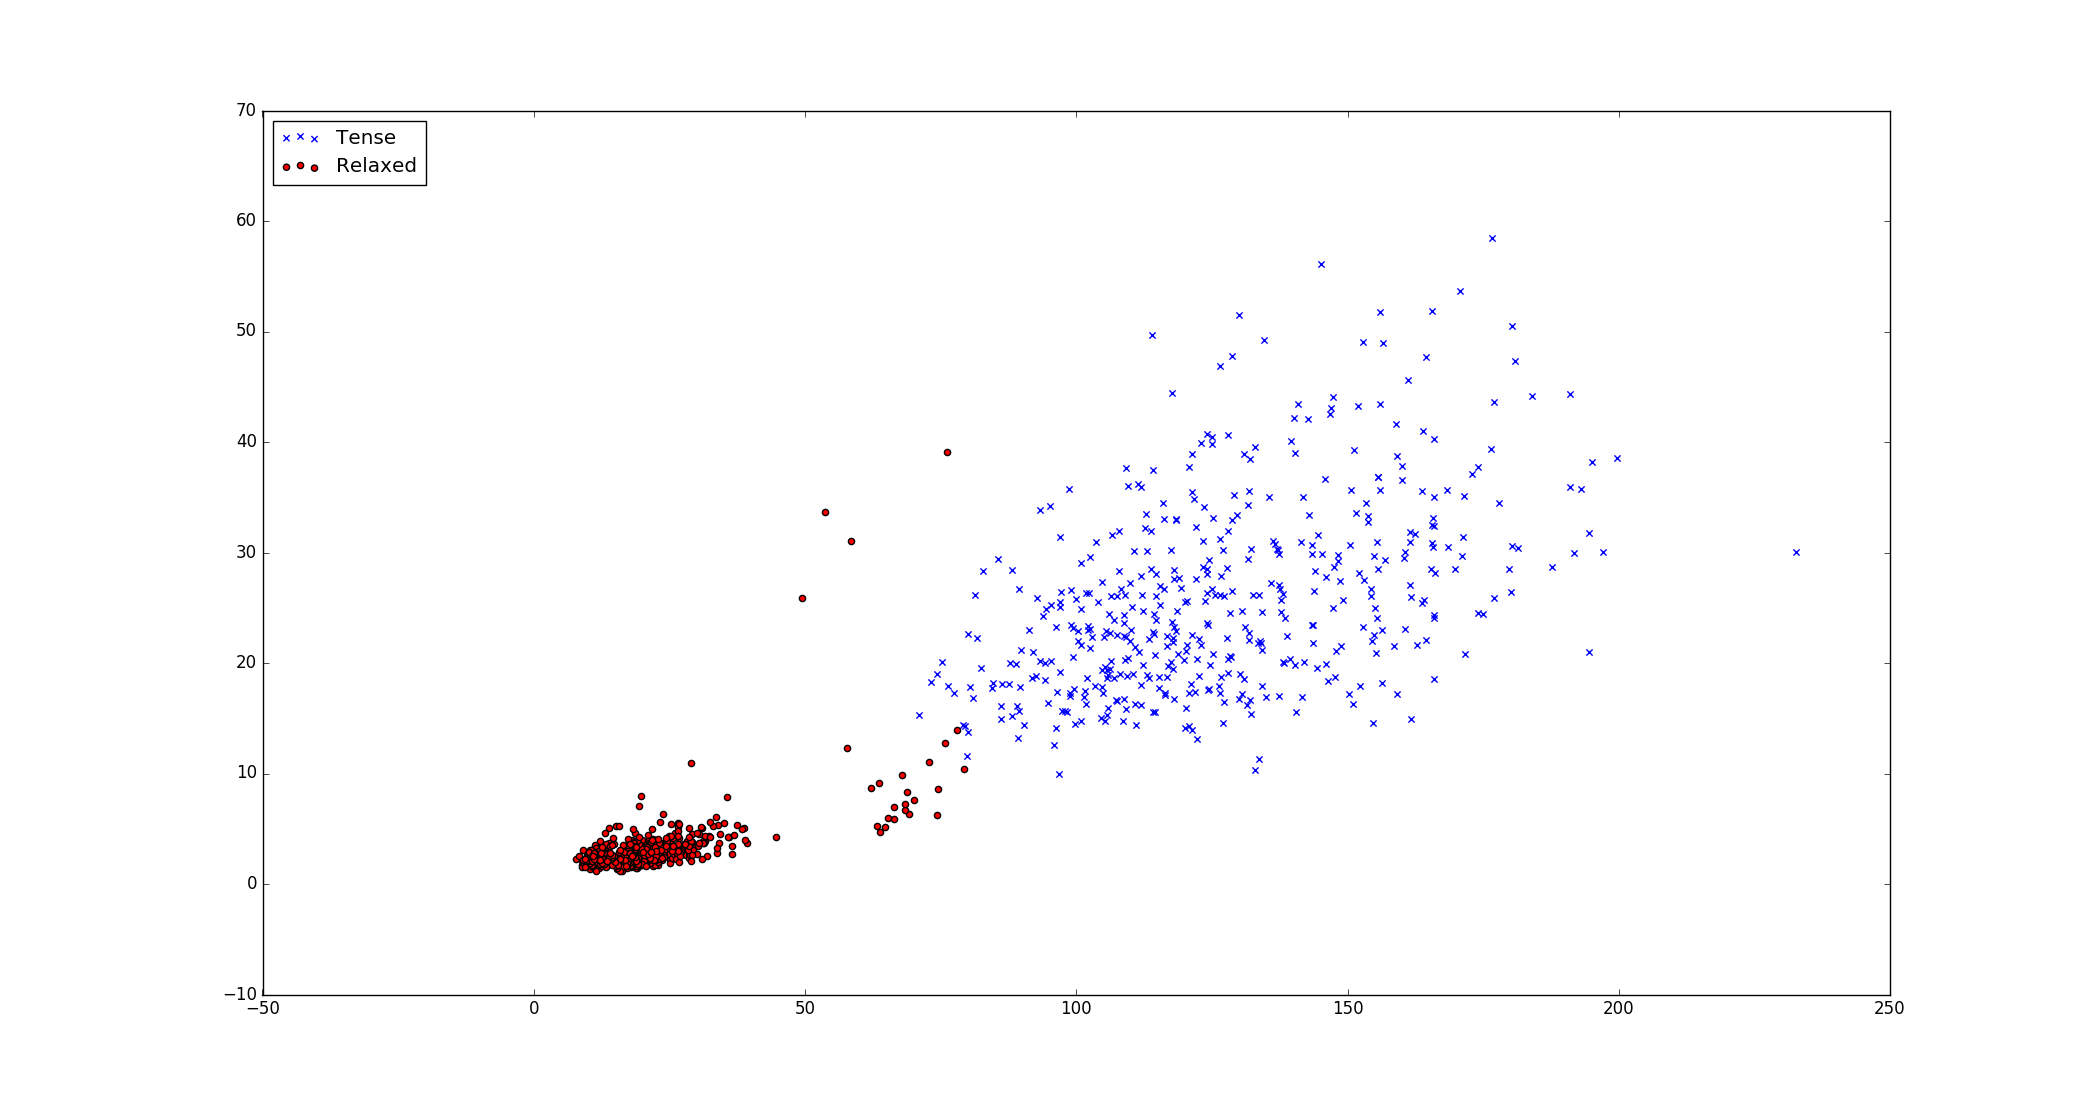
\includegraphics[width=1\textwidth]{javo-512-1.png}
    \caption{Gráfico de dispersión del vector de características EMG para la sesión del sujeto $3$ ($512\,Hz$).}
	\label{fig:emg-graph-s3-512}
\end{figure}

Las figuras \ref{fig:emg-graph-s1-512} y \ref{fig:emg-graph-s3-512} muestran, nuevamente, una clara separación entre las muestras tomadas durante el tiempo que se mantuvo el músculo relajado y tensado.

En definitiva, los niveles de precisión alcanzados utilizando las técnicas detalladas en este informe fueron muy elevados ($95\%$ o más en todos los casos). Éstos valores resultaron ser más que suficientes para el desarrollo de las simulaciones interactivas, que en sí también fueron diseñadas teniendo en cuenta que la precision de predicción prácticamente nunca podría ser del $100\%$.

La precisión fue tan alta, que en el universo interactivo, nunca se lanzó un proyectil prematuramente. Es decir, los proyectiles fueron siempre lanzados cuando el usuario lo deseó y no por accidente.

\section{\acrshort{spo2}}

Para medir la precision del método explicado en la sección \ref{sec:spo2-signal-processing}, se grabó una sesión de aproximadamente un minuto para cuatro sujetos, y se comparó el promedio de \acrshort{bpm} obtenido durante la duración del intervalo.

\begin{table}[H]
\centering
\begin{tabular}{ |c|c|c| } 
 \hline
 Sujeto & Promedio de \acrshort{bpm} (Sensor) & Promedio de \acrshort{bpm} (Calculado) \\ 
 \hline
 1 & $78.380$ & $77.055$ \\
 \hline
 2 & $84.300$ & $80.775$ \\
 \hline
 3 & $74.953$ & $73.848$ \\
 \hline
 4 & $80.412$ & $77.004$ \\

 \hline
\end{tabular}
\caption{Promedios de \acrshort{bpm} para las sesiones de \acrshort{spo2} medidas.}
\label{tab:spo2-results}
\end{table}

Como se puede ver en la tabla \ref{tab:spo2-results}, los resultados obtenidos a través de nuestro método de calculo de \acrshort{bpm} son similares a los calculados internamente por el sensor. La diferencia mas grande entre ambos resultados, para todas las sesiones, fue de aproximadamente $4\%$. Ambos métodos para calcular \acrshort{bpm} tienen sus ventajas y desventajas: el que utiliza el sensor produce valores que fluctúan menos en el tiempo, pero representan un valor promediado sobre un intervalo de tiempo extenso, por lo que no responden rápidamente a cambios en el ritmo cardíaco. Por el otro lado, nuestro método responde mas rápidamente a los cambios, pero tiende a producir resultados que fluctúan con mayores magnitudes. Se graficaron los resultados de las sesiones de los sujetos $2$ y $3$ para poder comparar visualmente los resultados:

\begin{figure}[H]
	\centering
    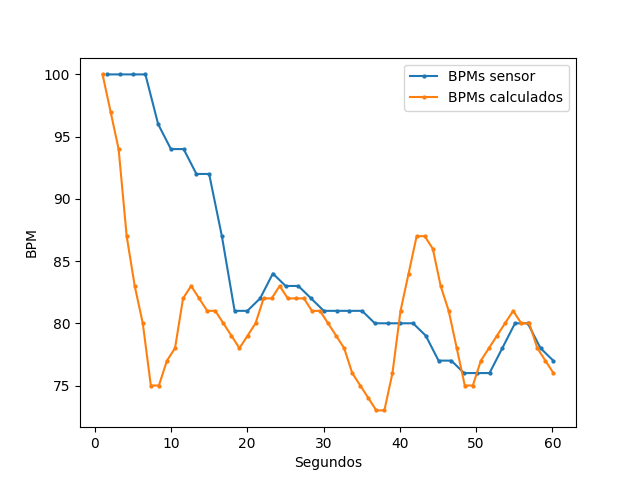
\includegraphics[width=0.8\textwidth]{javier-1-spo2.png}
    \caption{Gráfico de \acrshort{bpm} a través del tiempo para la sesión del sujeto $2$.}
	\label{fig:spo2-graph-2}
\end{figure}

\begin{figure}[H]
	\centering
    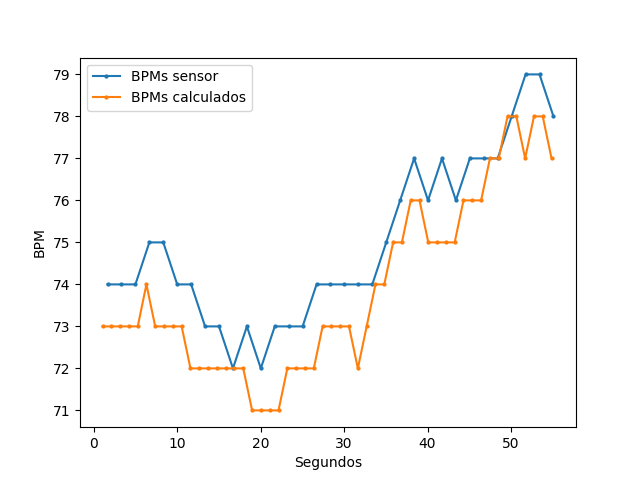
\includegraphics[width=0.8\textwidth]{gabriela-1-spo2.png}
    \caption{Gráfico de \acrshort{bpm} a través del tiempo para la sesión del sujeto $3$.}
	\label{fig:spo2-graph-3}
\end{figure}

El gráfico \ref{fig:spo2-graph-2} muestra como ambos métodos de medición tienden a producir los mismos resultados, pero con algunas diferencias. El método del sensor tiende a producir los mismos valores producidos por nuestro método, pero cierto atraso. A la vez, nuestro método tiende a producir resultados que varían mas rápidamente con el tiempo. El gráfico \ref{fig:spo2-graph-3} muestra una sesión donde ambos métodos produjeron resultados mucho mas similares. En el caso de éste proyecto, se prefirió nuestro método, ya que la simulación interactiva requiere de un tiempo de respuesta lo mas corto posible a los cambios de ritmo cardíaco del usuario. Es necesario remarcar que aunque las mediciones de \acrshort{bpm} son discretas, se utilizaron gráficos de línea ya que éstos permitían interpretar la información más fácilmente. Los valores leídos están representados como puntos sobre las líneas.

